\documentclass[10pt,a4paper]{article}
\usepackage[utf8x]{inputenc}
\usepackage{ucs}
\usepackage{amsmath}
\usepackage{amsfonts}
\usepackage{amssymb}
\usepackage{a4wide}
\usepackage{comment}
\usepackage[pdftex]{graphicx}
\usepackage{epstopdf}
\newcommand{\cmd}[1]{\texttt{#1}}
\newcommand{\remove}{}
\newcommand{\dir}[1]{\textsf{#1}}
\newcommand{\pop}{Depiler\xspace}
\newcommand{\push}{Empiler\xspace}
\newcommand{\tete}{LireTete}
\newcommand{\sommet}{LireSommet}
\newcommand{\empt}{EstVide}
\newcommand{\enqueue}{Enfiler\xspace}
\newcommand{\dequeue}{Defiler\xspace}
\newcommand{\get}{\ensuremath{\leftarrow\ }}

\usepackage[textsize=small, textwidth=2cm, color=yellow]{todonotes}


\usepackage{comment}
\usepackage{algorithm}
\usepackage[noend]{algpseudocode}
\usepackage{tcolorbox}

\newtcolorbox{mybox}[3][]
{
  colframe = #2!25,
  colback  = #2!10,
  coltitle = #2!20!black,  
  title    = {#3},
  #1,
}


\excludecomment{solution}
\includecomment{solution}

\title{IF111 - Algorithmes et structures de données-TD3 :\\ Graphes et représentations}
\date{}
\author{\underline{Jonathan Narboni}, Rohan Fossé}
\date{\underline{\texttt{jonathan.narboni@labri.fr}}, \texttt{rfosse@labri.fr}}


\begin{document}
\maketitle

\section*{Exercice 1}
Étant donné un tableau trié de n entiers distincts où chaque entier est compris entre 0 et m-1 et $m>n$. Recherchez le plus petit nombre manquant dans le tableau. Proposez un algorithme avec une complexité logarithmique $\mathcal{O}(log(n))$.\\
Par exemple, si l'on considère le tableau [0, 1, 2, 6, 9] avec n = 5 et m = 10, alors l'algorithme donnera 3.

\begin{tcolorbox}
def elementManquant(tab, debut, fin):\\
    if debut $>$ fin: \\
        return fin+1\\
     
    if debut != tab[debut]: \\
        return debut\\
 
    milieu = (debut+fin)//2\\
    if tab[milieu] == milieu:\\
        return elementManquant(tab, milieu+1, fin) \\
     
    return elementManquant(tab, debut, milieu)\\
\end{tcolorbox}

\section*{Exercice 2}
Écrire une fonction fusion qui prend en argument deux listes triées L1 et L2 et qui renvoie une seule liste triée contenant les éléments de L1 et L2.

\begin{tcolorbox}
On parcourt les deux listes en même temps afin de déterminer un premier rangement. On s'arrête lorsqu'une des deux listes est épuisée. On ajoute alors les termes qui restent de l'autre liste.

def fusion(L1,L2):\\
    n1=len(L1)\\
    n2=len(L2)\\
    i,j=0,0\\
    L=[]\\
    while ( (i<n1) and (j<n2)):\\
        if (L1[i]<L2[j]):\\
            L.append(L1[i])\\
            i=i+1\\
        else:\\
            L.append(L2[j])\\
            j=j+1\\
    On ajoute encore les termes de la liste non epuisee\\
    for i in range(i,n1):\\
        L.append(L1[i])\\
    for j in range(j,n2):\\
        L.append(L2[j])\\
    return L \\
\end{tcolorbox}

\section*{Exercice 3}
 Le graphe ci-dessous représente le plan d'une ville.\\

Le sommet A désigne l'emplacement des services techniques.\\

Les sommets B, C, D, E, F et G désignent les emplacements de jardins publics. Une arête représente l'avenue reliant deux emplacements et est pondérée par le nombre de feux tricolores situés sur le trajet. \\

\begin{figure}[h!]
    \centering
    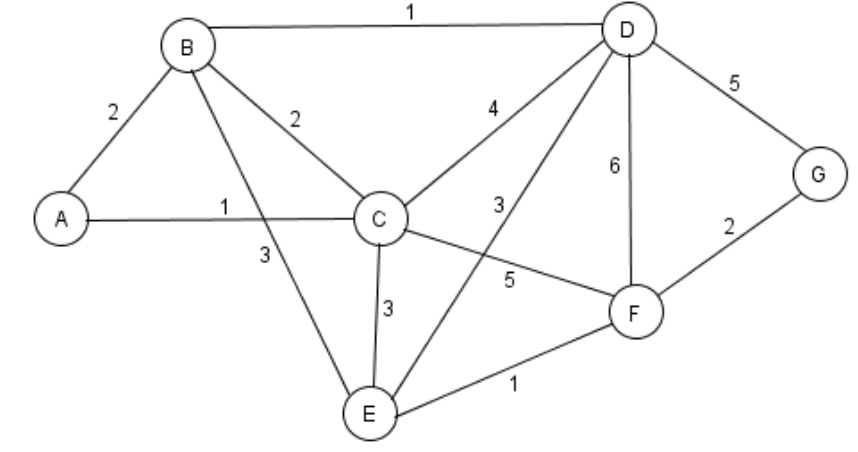
\includegraphics[scale=0.6]{Djisktra.png}
    \label{fig:my_label}
\end{figure}

 On s'intéresse au graphe non pondéré. Répondre aux questions suivantes :
\begin{enumerate}
    \item Ce graphe est-il connexe ?
    \item Ce graphe est-il complet ?
    \item Ce graphe admet-il une chaîne eulérienne ?
    \item Ce graphe admet-il un cycle eulérien ?
    \item Déterminer, en justifiant, le nombre chromatique de ce graphe.
\end{enumerate}
On s'intéresse dorénavant au graphe pondéré. Proposer un trajet comportant un minimum de feux tricolores reliant A à G.

\begin{tcolorbox}
\begin{enumerate}
    \item Le graphe est connexe car pour toute paire de sommets, il existe une chaîne reliant ces sommets.
    \item Le graphe n'est pas complet car les points A et D (par exemple) ne sont pas relié par une arête.
    \item D'après le théorème d'Euler, le graphe admet une chaîne eulérienne. En effet, il n'existe que deux sommets de degré impair(C et D)
    \item D'après le théorème d'Euler, le graphe n'admet pas de cycle eulérien. Il faudrait pour cela qu'il n'existe aucun sommet de degré impair
    \item BCDE forme un sous-graphe complet. Le nombre chromatique du graphe est donc supérieur ou égal à 4.
    On peut colorier le graphe avec 4 couleurs de la façon suivante (par exemple) :

rouge: A, D\\
bleu: B, F\\
vert: C, G\\
jaune: E\\

Le nombre chromatique du graphe est donc 4. 

\end{enumerate}

Avec Dijsktra, on voit que le minimum entre A et G est de 7 feux minimum (voir TD6 pour une correction détaillée).

\end{tcolorbox}


\section*{Exercice 4 (bonus)}
Soit un groupe de personnes tel que :
\begin{enumerate}
    \item Chaque personne est membre d’exactement deux associations;
    \item Chaque association comprend exactement trois membres;
    \item Deux associations quelconques ont toujours exactement un membre en commun.
\end{enumerate}
 
Combien y a-t-il de personnes ? d’associations ?

\begin{tcolorbox}
Supposons que nous avons n associations et considérons le graphe complet Kn dont les sommets représentent les associations (toute paire d’associations est donc reliée par une arête). Deux associations ayant toujours exactement un membre en commun, nous pouvons étiqueter l’arête reliant ces deux associations par le membre en question. Par ailleurs, chaque personne étant membre d’exactement deux associations, une même personne ne peut pas étiqueter deux arêtes distinctes (sinon elle appartiendrait à au moins trois associations). Les arêtes sont donc en bijection avec les personnes…\\

Finalement, chaque association comprenant exactement trois personnes, tous les sommets du graphe complet sont de degré 3. Il s’agit donc de K4 ! Le nombre d’associations est donc de 4 (nombre de sommets) et le nombre de personnes de 6 (nombre d’arêtes = 4 x 3 / 2).
\end{tcolorbox}

\end{document}

